% Compile with:
%     xelatex -file-line-error -halt-on-error -shell-escape lyse.tex
\documentclass[a4paper,11pt,titlepage]{article}
\pdfminorversion=5
\usepackage{cite}
\usepackage{lipsum}
\usepackage[pdftex]{graphicx}
\usepackage[font=small,format=plain,labelfont=bf,up,textfont=up]{caption}
\usepackage[top=3.5cm, bottom=4cm, left=4cm, right=4cm]{geometry}
\usepackage{setspace}
\usepackage{titlepic}
\usepackage{fancyhdr}
\usepackage[PetersLenny]{fncychap}
\usepackage{titlesec}
\usepackage{amsmath}
\usepackage{subfigure}
\usepackage{xcolor}
\usepackage[T1]{fontenc}
\usepackage{beramono}
\usepackage[urw-garamond]{mathdesign}
\usepackage{minted}
\usepackage{lettrine}

\newcommand{\python}[1]{\inputminted[linenos, numbersep=5pt, frame=lines, framesep=2mm,fontsize=\small]{python}{#1}}

\definecolor{pastelred}{RGB}{200,80,80}
\definecolor{pastelgreen}{RGB}{0,150,80}

% redefine \texttt to be coloured:
\renewcommand\texttt[1]{{\ttfamily\color{pastelgreen}#1}}

\usepackage[bookmarksopen, pagebackref]{hyperref}
\usepackage{doi}
\renewcommand*{\backref}[1]{}
\renewcommand*{\backrefalt}[4]{
  \ifnum#1=1
    [p~#2]
  \else
    [pp~#2]
  \fi
}

\hypersetup{
    colorlinks=true,%
    citecolor=pastelred,%
    filecolor=pastelred,%
    linkcolor=pastelred,%
    urlcolor=pastelred
}

\begin{document}

\title{\texttt{lyse}: a data analysis system for process-as-you-go automated data analysis}
\author{Chris Billington}
\maketitle
\tableofcontents
\section{Introduction}\label{sec:concepts}

\lettrine[lines=3]{\texttt{l}}{\texttt{yse}} is a data analysis system which gets \emph{your code } running on experimental data as it is acquired. It is fundamenally based around the ideas of experimental \emph{shots} and analysis \emph{routines}. A shot is one trial of an experiment, and a routine is a \texttt{Python} script, written by you, that does something with the measurement data from one or more shots.

Analysis routines can be either \emph{single-shot} or \emph{multi-shot}. This determines what data and functions are available to your code when it runs. A single-shot routine has access to the data from only one shot, and functions available for saving results only to the hdf5 file for that shot. A a multi-shot routine has access to the entire dataset from all the runs that are currently loaded into \texttt{lyse}, and has functions available for saving results to an hdf5 file which does not belong to any of the shots---it's a file that exists only to save the `meta results'.

Actually things are far less magical than that. The only enforced difference between a single shot routine and a multi-shot routine is a single variable provided to your code when \texttt{lyse} runs it. Your code runs in a perfectly clean \texttt{Python} environment with this one exception: a variable in the global namespace called \texttt{path}, which is a path to an hdf5 file. If you have told \texttt{lyse} that your routine is a singleshot one, then this path will point to the hdf5 file for the current shot being analysed. On the other hand, if you've told \texttt{lyse} that your routine is a multishot one, then it will be the path to an h5 file that has been selected in \texttt{lyse} for saving results to.

The other differences listed above are conventions only\footnote{Though \texttt{lyse}'s design is based around the assumption that you'll follow these conventions most of the time}, and pertain to how you use the API that \texttt{lyse} provides, which will be different depending on what sort of analysis you're doing.

Here's a screenshot of \texttt{lyse}:

\begin{center}
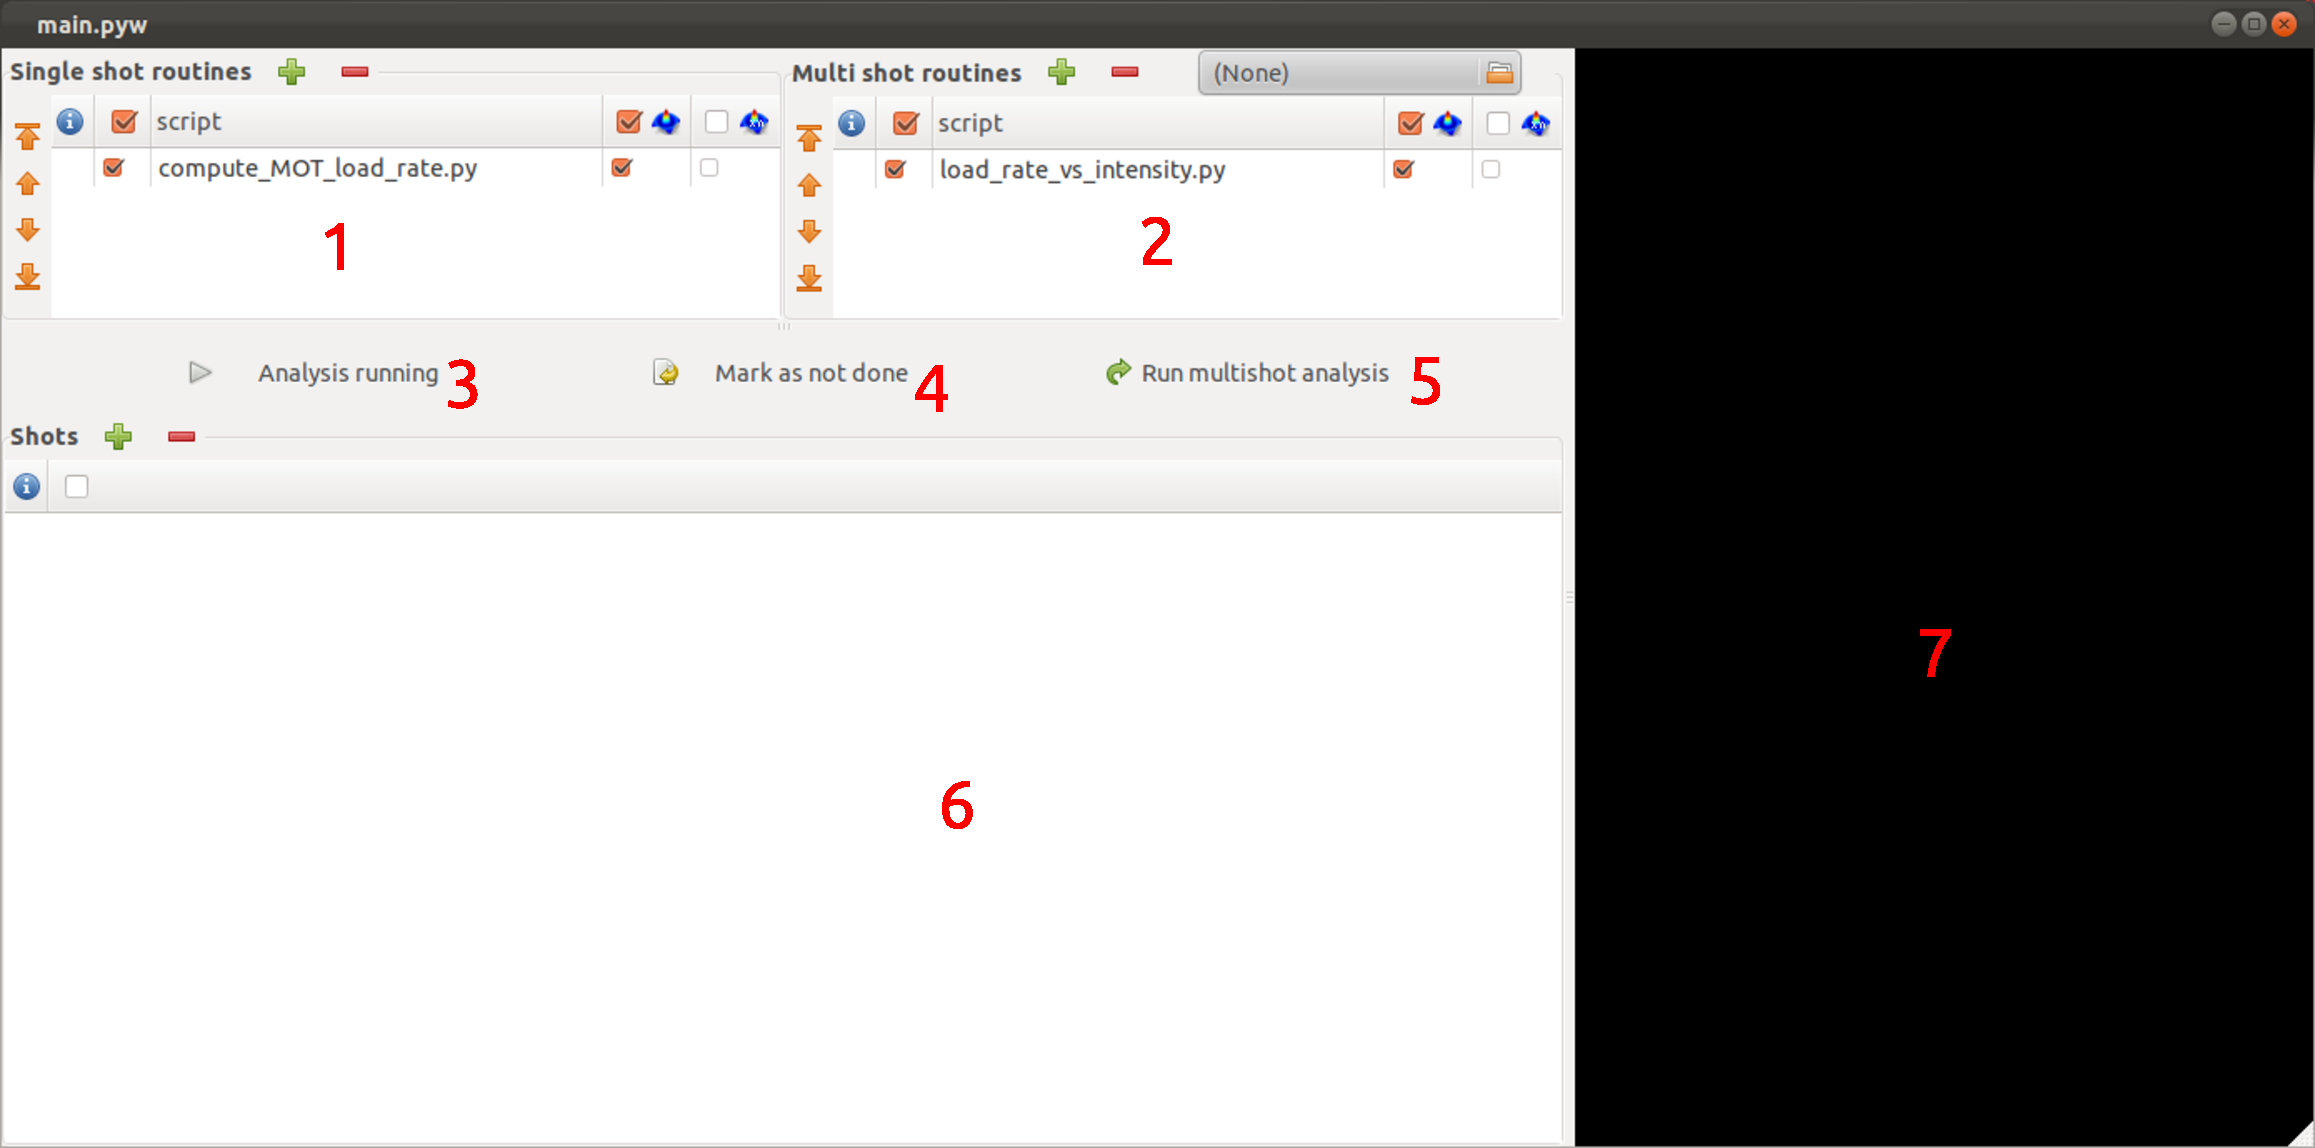
\includegraphics[width=\textwidth]{gui.pdf}
\end{center}

\begin{enumerate}
\item Here's where single shot routines can be added and removed, with the plus and minus buttons. They will be executed in order on each shot (more on how that works shortly). They can be reordered, or enabled/disabled with the checkboxes on the left. The checkboxes to the right, underneath the plot icons don't currently do anything, but they are intended to provide control over how plots generated by the analysis routines are displayed and updated.

\item Here is where multi-shot routines can be added or removed. The file selection button at the top allows you to select what hdf5 file multi-shot routines will get given (to which they will save their results).

\item Allows pausing of analysis. \texttt{lyse} by default will run all single-shot routines on a shot when it arrives (either via the HTTP server or having been manually added). After all the shots have been processed, only then will the multi-shot routines be executed. So if you load ten shots in quickly, the multi-shot routines won't run until they've all been processed by the single-shot routines. However most of the time there will be sufficient delay in between shots arriving that multi-shot routines will be executed pretty much every time a new shot arrives.

\item If you want to re-run single-shot analyses on some shots, select them and click this button. They'll then be processed in order.

\item This will rerun all the multi-shot analyses.

\item Here is where shots appear, either having arrived over HTTP of having been added manually via the file browser (by clicking the plus button). Many columns will populate this part of the screen, one for each global and each of the results (as saved by single-shot routines) present in the shots. A high-priority planned feature is to be able to choose exactly which globals and results are displayed. Otherwise this display is overwhelming to the point of uselessness. The data displayed here represents the entirety of what is available to multi-shot routines via the API provided by \texttt{lyse}.

\item This is where the output of routines is displayed, errors in red. If you're putting \texttt{print} statements in your analysis code, here is where to look to see them. Likewise if there's an exception and analysis stops, look here to see why.
\end{enumerate}

\section{The \texttt{lyse} API}
\lettrine[lines=3]{S}{o great,}  you've got a single filepath. What data analysis could you possibly do with that? It might seem like you have to still do the same amount of work that you would without an analysis system! Whilst that's not quite true, it's intentionally been designed that way so that you can run your code outside \texttt{lyse} with very little modification. Another motivating factor is to minimise the amount of magic black box behaviour, such that an analysis routine is actually just an ordinary \texttt{Python} script which makes use of an API designed for our purposes. \texttt{lyse} is both a program which executes your code, and an API that your code can call on.

To get started, you'll want to begin your analysis routine with:
\python{listing_1.py}

The \texttt{lyse} module\footnote{importing lyse imports the functions in \texttt{pythonlib/lyse/\_\_init\_\_.py}, whereas the main program is \texttt{pythonlib/lyse/main.pyw}} provides the following one function and two classes:
\begin{description}
\item[\texttt{data(filepath=None, host='localhost')}]. The \texttt{data} function when called with no arguments obtains the current dataset from a running instance of \texttt{lyse} on the same computer. It returns a \texttt{pandas} \texttt{DataFrame} with the same rows and columns as you see in the main program of \texttt{lyse}. This is a simple way to get at your data, that doesn't require at all that your code is being run from within \texttt{lyse}. You can simply open a python interactive session, type \texttt{from lyse import *; df = data()}, and begin pulling out columns and plotting them against each other. Callin \texttt{data()} this way is intended for pulling data for multi-shot analysis, and should be avoided in single-shot mode. 

When called with the \texttt{host} argument, the \texttt{data} function instead connects to a running instance of \texttt{lyse} on that computer, downloading its \texttt{DataFrame} over the network. I'm planning on including automatic \texttt{SSH} tunnelling through \texttt{bec.physics} to allow for us to obtain our data from outside the lab subnet without the need for a VPN.

When called with the \texttt{filepath} argument, the \texttt{data} function instead returns a \texttt{pandas Series} object with the globals and results from just the h5 file specified. This is intended for use in single-shot mode, with the filepath being that single global variable that \texttt{lyse} implants into the namespace, as I mentioned in sec \ref{sec:concepts}.

\item[\texttt{Run(h5\_path)}]\footnote{There is another argument to this function---\texttt{no\_write=False}, but is is intended for use only internally by \texttt{Sequence}, which instantiates many runs but disables their functions for writing to file} Sometimes you need more than just the globals and results in single shot mode. In fact, you cannot produce any results without having access to measurement data---that is traces and images. Run objects provide methods for obtaining this data from an h5 file. They also provide methods for saving your results back to the same h5 file. 

\begin{description}
\item[\texttt{t, V = Run.get\_trace(name)}] Returns an array of times and an array of voltages for an analogue input trace named \texttt{name}, as specified in a call to \texttt{AnalogIn.acquire} in \texttt{labscript}.

\item[\texttt{im = Run.get\_image(orientation,label,image)}] Returns an image (as an array) from the camera with specified orientation (eg \emph{side}, \emph{top}), image label (eg \emph{fluorescence}, \emph{absorption}), and specific image name (eg \emph{OD}, \emph{atoms}, \emph{flat}).

\item[\texttt{Run.save\_result(name,value)}] Saves a single-value result to the hdf5 file. The result will be saved as an attribute to the group \texttt{/results/} \texttt{your\_script's\_filename}, with the attribute \texttt{name} . Results saved in this way will be available to subsequent routines in the \texttt{DataFrame}s and \texttt{Series} returned by \texttt{data()} under the hierarchy \texttt{dataframe[your\_script's\_ filename, your\_result's\_name]}.

\item[\texttt{Run.save\_result\_array(name,data)}] This method saves an array which can be any numpy datatype convertible to hdf5 datatypes (which is pretty much any numpy array, including numpy `record' arrays---those are the ones with named columns). The array will be saved in a dataset under the group \texttt{/results/} \texttt{your\_script's\_filename}, with the dataset's name being \texttt{name}. It will not be accessible alongside globals and single-value results, but can be accessed with the \texttt{get\_result\_array} method.

\item[\texttt{arr = Run.get\_result\_array(group,name)}] This returns a numpy array as saved by the \texttt{save\_result\_array} function. The \texttt{group} argument specifies the name of the group that the result array was saved to within the results group of the hdf5 file. This will be then filename of the analysis routine which saved the result. 

\item[\texttt{Run.set\_group(groupname)}] When running \texttt{Python} in interactive mode, the \texttt{Run} object can't know what filename to use as the hdf5 group name to which results are saved with \texttt{save\_result} and \texttt{save\_result\_array}. So if you try to instantiate a \texttt{Run} object in interactive mode, you'll be prompted to call this method to set what the group name should be instead.

\item[\texttt{t1, V1,...tn, Vn = Run.get\_trace(name\_1,..., name\_n)}]\ 

A convenience method for getting many traces at once.

\item[\texttt{Run.save\_results(name\_1,value\_1..., name\_n, value\_n)}]\ 

A convenience method for saving many results at once.

\item[\texttt{arr1,...arrn = Run.get\_result\_arrays(group, name\_1,..., name\_n)}]\ 

A convenience method for getting many result arrays at once, provided they are within the same group.

\item[\texttt{Run.save\_result\_arrays(name\_1,data\_1..., name\_n, data\_n)}]\ 

A convenience method for saving many result arrays at once.

\end{description}
\item[\texttt{Sequence(h5\_path,run\_paths)}] A \texttt{Sequence} object represents many runs. It provides methods for getting data from the runs, and for saving the results of multi-shot analyses to the file specified by \texttt{h5\_path}, which should be the filepath that \texttt{lyse} provides to your multi-shot analysis script. \texttt{run\_paths} should be a list of filepaths that you would like to be included in this \texttt{Sequence}. You can pull out these filenames from the \texttt{DataFrame} provided by the \texttt{data()} function with \texttt{df['filepaths']}. You might use this to pass in the filepaths for only a subset of the shots. You can also pass in the entire \texttt{DataFrame} as the \texttt{run\_paths}, and if it contains a column called \texttt{'filepaths'}, then those filepaths will be used.

\begin{description}
\item[\texttt{Sequence.runs}] The sequence object contains a \texttt{Run} object for each of the files in \texttt{run\_paths}.  \texttt{Sequence.runs} is a dictionary of these \texttt{Run} objects, keyed by filepath. This dictionary is mainly for internal use by the \texttt{Sequence} object, but is included here in case you really do need to delve into the data from individual shots during a multi-shot routine. All methods of these \texttt{Run} objects that would write to their hdf5 file have been disabled.

\item[\texttt{Sequence.get\_result\_array}] Takes the same arguments as \texttt{Run.get\_result\_array}, and returns a dictionary of result arrays, one for each run, keyed by filepath.

\item[\texttt{Sequence.get\_trace}]Takes the same arguments as \texttt{Run.get\_result\_array}, and returns a dictionary of t, V tuples, one for each run, keyed by filepath.


\end{description}

The \texttt{Sequence} object also has the methods \texttt{save\_result}, \texttt{save\_result\_array}, \texttt{save\_results} and \texttt{save\_result\_arrays}, which work identically to equivalent methods in the \texttt{Run} object\footnote{\texttt{Sequence} is actually a subclass of \texttt{Run}}, the only difference being that you're saving the results to the h5 file associated with the \texttt{Sequence} object, rather than a file associated with a single shot.

\end{description}


\section{Examples}
\subsection{Single-shot example}

\python{listing_2.py}

\subsection{Multi-shot example}

\python{listing_3.py}

\end{document}
